\begin{figure*}[htb]
\vspace*{0.06in}
  \centering
  \begin{minipage}{0.22\textwidth}
  \centering
  \begin{tikzpicture}[inner sep=0pt,outer sep=0pt]
    \node[anchor=south west] (comp1) at ($(0, 0)$)
    	{{\includegraphics[height=1.4in]{figs/sce1.png}}};
    \node[anchor=north] at ($(comp1.south)+(0,-0.3)$) {\centering Sector};
  \end{tikzpicture}%
  \end{minipage}
  \hfill
  \begin{minipage}{0.22\textwidth}
  \centering
  \begin{tikzpicture}[inner sep=0pt,outer sep=0pt]
    \node[anchor=south west] (comp2) at ($(0, 0)$)
    	{{\includegraphics[height=1.4in]{figs/sce2.jpg}}};
    \node[anchor=north] at ($(comp2.south)+(0,-0.3)$) {\centering Dense};
  \end{tikzpicture}%
  \end{minipage}
  \hfill
  \begin{minipage}{0.22\textwidth}
  \centering
  \begin{tikzpicture}[inner sep=0pt,outer sep=0pt]
    \node[anchor=south west] (comp2) at ($(0, 0)$)
    	{{\includegraphics[height=1.4in]{figs/sce3.png}}};
    \node[anchor=north] at ($(comp2.south)+(0,-0.3)$) {\centering Campus};
  \end{tikzpicture}%
  \end{minipage}
  \hfill
  \begin{minipage}{0.3\textwidth}
  \centering
  \begin{tikzpicture}[inner sep=0pt,outer sep=0pt]
    \node[anchor=south west] (comp2) at ($(0, 0)$)
    	{{\includegraphics[height=1.4in]{figs/sce4.png}}};
    \node[anchor=north] at ($(comp2.south)+(0,-0.3)$) {\centering Office};
  \end{tikzpicture}%
  \end{minipage}
  \caption{Four simulation scenarios. In sector and campus worlds, start region/poses (red) and end region/poses (green) are labeled. In the dense world, robot navigates from top to bottom. In the office world, the start and goal poses are randomly chosen from the red points. \label{fig:sim}}
  \vspace*{-0.5em}
\end{figure*}

\begin{figure*}[!htb]
% \vspace*{-0.5em}
\begin{minipage}{0.3\textwidth}
\centering
\captionsetup{justification=centering}
\captionof{table}{ STDR Simulation Benchmark \\ ($1^{\text{st}}$ order nonholonomic model)\label{tab:sim_ben_s}}
% \vspace{2in}
\begin{tikzpicture}[inner sep=0pt,outer sep=0pt,scale=1, every node/.style={scale=1}]
    \node[anchor=west] (sim_stdr) at ($(0, 0pt)$)
    {
    \setlength{\tabcolsep}{4pt}
    \begin{tabular}{|c||ccc|}
    \hline 
    \textbf{Total} & Success & Abort & Collision \\ 
    \hline 
    PG & 100\%  & 0\%  & 0\%  \\ 
    SG & 100\%  & 0\%  & 0\%  \\ 
    \hline 
    \end{tabular}
    };

\end{tikzpicture}
\end{minipage}
\hfill
\begin{minipage}{0.3\textwidth}
\centering
\captionsetup{justification=centering}
\captionof{table}{ Gazebo Simulation Benchmark \\ ($2^{\text{nd}}$ order nonholonomic model)\label{tab:sim_ben_g}}
% \vspace{2in}
\begin{tikzpicture}[inner sep=0pt,outer sep=0pt,scale=1, every node/.style={scale=1}]
    \node[anchor=west] (sim_stdr) at ($(0, 0pt)$)
    {
    \setlength{\tabcolsep}{4pt}
    \begin{tabular}{|c||ccc|}
    \hline 
    \textbf{Total} & Success & Abort & Collision \\ 
    \hline 
    PG & 91\%  & 8\%  & 1\%  \\ 
    SG & 100\%  & 0\%  & 0\%  \\
    \hline 
    \end{tabular}
    };

\end{tikzpicture}
\end{minipage}
\hfill
\begin{minipage}{0.38\textwidth}
\centering
  \scalebox{0.75}{
  \begin{tikzpicture}[inner sep=0pt,outer sep=0pt]
    \node[anchor=south west] at ($(0, 0)$)
    	{{\includegraphics[height=1.1in]{figs/sim_comp.png}}};
  \end{tikzpicture}%
  }
  \caption{Success rates comparison between PG and SG. \label{fig:sim_comp}}
\end{minipage}
\vspace*{-1em}
\end{figure*}

\begin{figure*}[!htb]
\vspace*{-0.5em}
\begin{minipage}{\textwidth}
\centering
\vspace*{0.1in}
\captionof{table}{ Simulation results in 4 Gazebo scenarios \label{tab:sim_ben_r}}
% \vspace{2in}
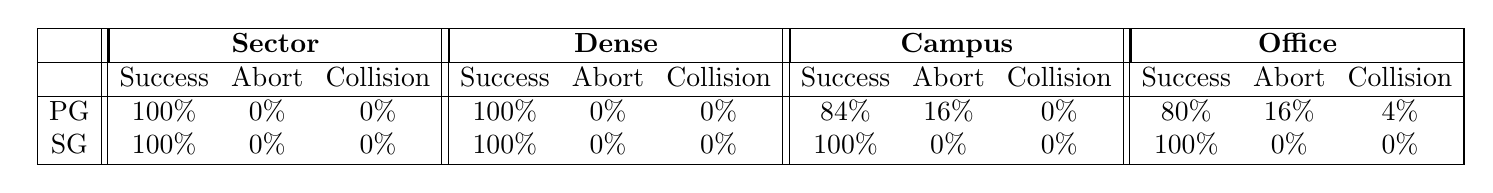
\begin{tikzpicture}[inner sep=0pt,outer sep=0pt,scale=1, every node/.style={scale=1}]

	\node[anchor=north west] (sim_dense) at (0, 0pt)
    {
    \setlength{\tabcolsep}{4pt}
    \begin{tabular}{|c||ccc||ccc||ccc||ccc|}
    \hline 
    & \multicolumn{3}{|c||}{\textbf{Sector}} & \multicolumn{3}{|c||}{\textbf{Dense}} & \multicolumn{3}{|c||}{\textbf{Campus}} & \multicolumn{3}{|c|}{\textbf{Office}} \\
    \hline
     & Success & Abort & Collision & Success & Abort & Collision & Success & Abort & Collision & Success & Abort & Collision \\ 
    \hline 
    PG & 100\%  & 0\%  & 0\%  & 100\%  & 0\%  & 0\% & 84\%  & 16\%  & 0\% & 80\%  & 16\%  & 4\% \\ 
    SG & 100\%  & 0\%  & 0\% & 100\%  & 0\%  & 0\% & 100\%  & 0\%  & 0\% & 100\%  & 0\%  & 0\%  \\ 
    \hline 
    \end{tabular}
    };

\end{tikzpicture}
\end{minipage}
% \vspace*{-1em}
\end{figure*}

\begin{figure*}[!htb]
  \centering
  \begin{minipage}{0.32\textwidth}
  \centering
  \begin{tikzpicture}[inner sep=0pt,outer sep=0pt]
    \node[anchor=south west] (comp1) at ($(0, 0)$)
    	{{\includegraphics[height=1.25in]{figs/s1_trace.png}}};
    \node[anchor=north] at ($(comp1.south)+(0,-0.3)$) {\centering Low Density};

    \node[anchor=north,color=yellow] at ($(comp1.south)+(-2.3,1.8)$) {\centering \Large \textbf{Start}};
    \node[anchor=north,color=yellow] at ($(comp1.south)+(2.3,1.8)$) {\centering \Large \textbf{Goal}};
  \end{tikzpicture}%
  \end{minipage}
  \hfill
  \begin{minipage}{0.32\textwidth}
  \centering
  \begin{tikzpicture}[inner sep=0pt,outer sep=0pt]
    \node[anchor=south west] (comp2) at ($(0, 0)$)
    	{{\includegraphics[height=1.25in]{figs/s3_trace.png}}};
    \node[anchor=north] at ($(comp2.south)+(0,-0.3)$) {\centering Medium Density};

    \node[anchor=north,color=yellow] at ($(comp1.south)+(-2.3,1.8)$) {\centering \Large \textbf{Start}};
    \node[anchor=north,color=yellow] at ($(comp1.south)+(2.3,1.8)$) {\centering \Large \textbf{Goal}};
  \end{tikzpicture}%
  \end{minipage}
  \hfill
  \begin{minipage}{0.32\textwidth}
  \centering
  \begin{tikzpicture}[inner sep=0pt,outer sep=0pt]
    \node[anchor=south west] (comp2) at ($(0, 0)$)
    	{{\includegraphics[height=1.25in]{figs/s5_trace.png}}};
    \node[anchor=north] at ($(comp2.south)+(0,-0.3)$) {\centering High Density};

    \node[anchor=north,color=yellow] at ($(comp1.south)+(-2.3,1.8)$) {\centering \Large \textbf{Start}};
    \node[anchor=north,color=yellow] at ($(comp1.south)+(2.3,2.5)$) {\centering \Large \textbf{Goal}};
  \end{tikzpicture}%
  \end{minipage}
  \caption{Real experiment topview. Three environment densities are shown. The green paths are the robot's real traces. Robots start from left to the right. \label{fig:real}}
  \vspace*{-0.5em}
\end{figure*}

To test navigation performance with {\saferGap}, simulation benchmark and real robot experiments are conducted.

\subsection{Simulation Benchmark}

\subsubsection{Simulation Configuration}
We benchmarked {\saferGap} local planer in ROS with move\_base hierarchical navigation system.  The benchmark is performed in both STDR and Gazebo simulators. STDR uses $1^{\text{st}}$ order circular nonholonomic model with 360$^\circ$ Field-of-View (FoV) laser scanner. In Gazebo, Turtlebot is used as the $2^{\text{nd}}$ order nonholonomic mobile robot with limited 60$^\circ$ FoV. We setup four different scenarios \cite{Smith2020} in Fig.~\ref{fig:sim} for benchmark: sector, dense, campus, and office. They simulate multiple navigation environments, e.g. hallway, open area with obstacles, campus roads and etc. The obstacles are randomly spawned in the scenarios with a minimum distance to each other as 1m. Robot start and end poses are also randomly chosen in the designated areas. Ground truth robot locations are used for navigation.  We have 50 Monte Carlo runs for each scenario to quantitatively compare {\saferGap} (SG) navigation performance with {\pGap} (PG) which serves as the baseline method. Radial extension and projection operator are enabled in PG for nonholonomic robot.

\subsubsection{Evaluation Metric}

Success, abort and collision rates are collected for each planner. Success means that the robot can successfully reach the goal. Abort represents that the robot cannot have any possible plan to the goal after recovery behavior. Collision is counted whenever a colliding happens.  

\subsubsection{Simulation Results}

The overall simulation results of STDR and Gazebo are in Table~\ref{tab:sim_ben_s} and \ref{tab:sim_ben_g}. The comparison of success rates is in Fig.~\ref{fig:sim_comp}. Both PG and SG have 100\% success rates in STDR with full sensing of the environments. However, when simulating $2^{\text{nd}}$ order nonholonomic model with limited FoV, PG's success rate drops 9\% including 8\% aborts and 1\% collisions. 

From the full results of 4 Gazebo scenarios in Table~\ref{tab:sim_ben_r}, PG does not perform well in the hallway and campus roads. The robot navigates back and forth, and is stuck to find successful paths to the goal. The projection operator in PG conservatively keep safety by sacrificing passibility. Due to the limited FoV, the PG still has collisions when all nonholonomic extensions are enabled. Our proposed local planner SG not only maintains safety, but also leverages the line-of-sight visible gaps for passibility. This comparison demonstrates safety guarantee for nonholonomic mobile robots in the design of {\saferGap}.

\subsubsection{Computational Efficiency}

The benchmark is performed on a workstation with Intel i7-8700. CasADi optimization framework is used for solving NMPC. We set the number of horizon $N=6$. The total time of each control loop is averaged as $\sim 75ms$, including B\'{e}zier path synthesis, keyhole generation, NMPC optimization, and CBF-QP. Real time application is achievable.



\subsection{Real Experiments}

The simulation benchmark quantitatively compares {\saferGap} navigation performance with {\pGap}, and presents the outperforming results of our proposed work. In this section, the planner is applied on the real platform, LoCoBot, to navigate through unknown environments. It has a Kobuki base with nonholonomic dynamics. Robot's odometry provides the pose information. RealSense D435i depth camera initially produces depth images that are converted to laserscan measurements through a ROS package depthimage\_to\_laserscan \cite{depthToLaser}.

We test {\saferGap} local planner in five scenarios with different obstacle densities from low to high in Fig.~\ref{fig:real}. The robot navigation traces are depicted on the top-view figures. For each configuration, 2 runs are repeated to show consistent results. We have 100\% success rate in totally 10 trials, which is the same as simulation. Therefore, {\saferGap} local planner is applicable on the real nonholonomic robots to maintain navigation safety and passibility.

